\section{W6: Software Quality Management}

\textbf{1. Understand the fundamentals of quality management}: 

    \textbf{1.1. What is Software Quality}: Seen from two aspects, end-user perspective (external quality characteristics) and developer perspective (internal quality characteristics). 

    \textbf{1.2. Cost of Software Quality}: Cost of Conformance (delivering products that meet requirements and are fit for purpose) and Cost of Non-Conformance (refers to taking responsibility for failures or not meeting quality expectations).

\textbf{2. Quality management processes}

    \textbf{2.1. Quality Assurance}: process is primarily concerned with defining or selecting the quality standards. Standards are a set of rules for ensuring quality.

        \textbf{2.1.1. Verification and Validation}: Verification is an attempt to ensure that the product is built correctly, i.e. building the system right. Validation is an attempt to ensure that the product is built according to the user's needs, i.e. building the right system.

        \textbf{2.1.2. Types of Testing}: unit test (smallest unit of testing), integration test (ensures subset of system work correctly together), system test (test entire system is working correctly), user acceptance test.

        \textbf{2.1.3. Standards (ISO Standards, Document Standards, Process Standards, Product Standards)}

        \textbf{2.1.4. Capability Maturity Model Integration}
        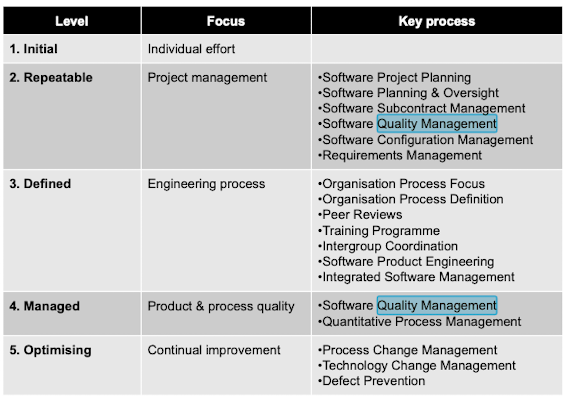
\includegraphics[width=\linewidth]{figs/SCR-20240606-orfm.png}

        \textbf{2.1.5. McCall Quality Model.}
        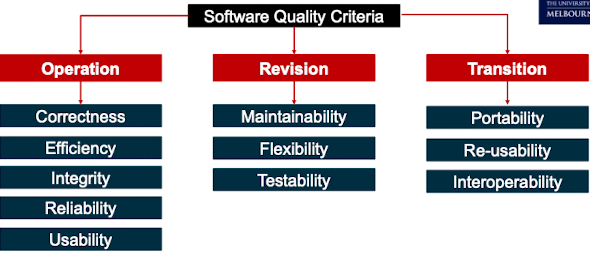
\includegraphics[width=\linewidth]{figs/SCR-20240606-orsk.png}
        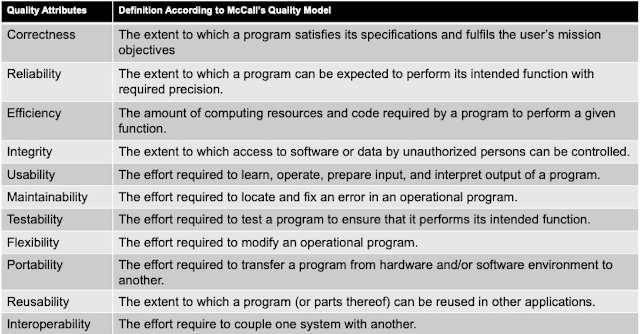
\includegraphics[width=\linewidth]{figs/SCR-20240606-osms.png}

    \textbf{2.2. Quality Planning.}

        \textbf{2.2.1. Software Quality Plan}: Product overview (a description of the product, intended market, and quality expectations), product plan (the critical release dates and responsibilities), quality goals (and plans for the product, including identification and justification of critical product quality attributes), process description (the quality assurance processes that should be used for the product development and management), document and coding standards, and risks and risk management.

        \textbf{2.2.2. Quality Control and Monitoring.}

        \textbf{2.2.3. Technical Reviews.}

        \textbf{2.2.4. Business Reviews}: The goal is to ensure that the IT solution provides the functionality specified in the project scope and requirements document.

        \textbf{2.2.5. Management Reviews}: compares the project's actual progress against a baseline project plan.
